\documentclass[a4paper,10pt]{article}
\usepackage[utf8]{inputenc}
\usepackage{polski}
\usepackage{graphicx}
\usepackage{listings}
\usepackage[usenames,dvipsnames]{color}
\addtolength{\hoffset}{-1cm}
\addtolength{\voffset}{-2cm}
\addtolength{\textwidth}{2cm}
\addtolength{\textheight}{3cm}
\usepackage{setspace}
\usepackage{indentfirst}
\usepackage{graphicx}
\lstset{
    language=Matlab,
    basicstyle=\scriptsize,
    aboveskip={1.5\baselineskip},
    columns=fixed,
    showstringspaces=false,
    extendedchars=true,
    breaklines=true,
    tabsize=4,
    prebreak = \raisebox{0ex}[0ex][0ex]{\ensuremath{\hookleftarrow}},
    frame=single,
    showtabs=false,
    showspaces=false,
    showstringspaces=false,
    identifierstyle=\ttfamily,
    keywordstyle=\color[rgb]{0,0,1},
    commentstyle=\color[rgb]{0.133,0.545,0.133},
    stringstyle=\color[rgb]{0.627,0.126,0.941},
    numbers=left,
    numberstyle=\tiny,
    stepnumber=1,
    numbersep=5pt,
    captionpos=b,
    escapeinside={\%*}{*)}
}

\def\figurename{Rys.}
\def\lstlistingname{Fun.}

\title{Informatyczne Systemy Sterowania \\ \large Ćwiczenie 4: Sterowanie szybkością transmisji w sieci komputerowej}

\author{Krzysztof Przybylski 239266}

\begin{document}
\maketitle
\section{Wstęp}\label{sec:wstęp}
\subsection{Cel ćwiczenia}
Wykonanie symulacji systemu sterowania ruchem w sieci komputerowej celem: \\
\begin{enumerate}
	\item Poznania problemu sterowania ruchem w sieci komputerowej jako przykładu 
sterowania systemem komputerowym. 
	\item Nabycia umiejętności wykorzystania pakietu Matlab oraz Simulink do symulacji ww. systemu. 
\end{enumerate}
\subsection{Plan działań} 
\begin{enumerate}
	\item Symulacja systemu sterowania szybkością transmisji.
	\\W trakcie realizacji zadania należy zamodelować obiekt sterowania (mechanizmy sieci
	komputerowej uwzględniane w problemie sterowania ruchem w sieci komputerowej).
	
	\item Dobór optymalnego regulatora.
	\\Realizacja zadania polega na
	\begin{enumerate}
		
		\item Doborze odpowiedniej struktury urządzenia sterującego z grupy regulatorów PID (P,
		PI, PD, PID).	
		\item Doborze optymalnych wartości parametrów regulatora.
		\item Przeprowadzeniu badań pozwalających na ocenę jakości działania rozpatrywanego
		systemu.
	\end{enumerate}
	
	\item Zastosowanie członów korekcyjnych.
	\\Realizacja zadania polega na:
	\begin{enumerate}
		
		\item Zaproponowaniu zastosowania odpowiednich członów korekcyjnych, pozwalających
		na polepszenie jakości działania systemu.
		\item Przeprowadzeniu symulacji działania systemu z takimi członami.
		\item Dobraniu optymalnych wartości parametrów członu korekcyjnego.
	\end{enumerate}
\end{enumerate}
\section{Realizacja planu i wyniki}

%-------------------------------------------------------------------------------------
%                                ZADANIE 1
%-------------------------------------------------------------------------------------
\subsection{Symulacja systemu sterowania szybkością transmisji}
Systemem symulowanym w tym ćwiczeniu będzie system opisany w artykule "\textit{Complete Stability Region
	Characterization for PI-AQM}" podanym w literaturze. Jest to sieć, w której:
\newline $C$ - przepustowość sieci,\newline $N$ - ilość otwartych sieci TCP,\newline  $d$ - opóźnienie pakietów, uzyskaliśmy następującą transmitancję.

\begin{equation} \label{eqn:transO}
P(s)={B \over (s + \alpha) (s + \beta)}e^{-sd}
\end{equation}

Gdzie $\alpha = {2N \over d^{2}C}$, $\beta = {1 \over d}$ i $B = {C^2 \over 2N}$.\\

Do regulowania systemu będę używał regulatorów z rodziny PID.
\newline\newline Żeby zasymulować system w Simulinku pomnożyłem mianownik transmitancji obiektu tak, aby można było wykorzystać go w bloku LTI system.
\begin{equation} \label{eqn:transO}
P(s)={B \over s^{2} + (\alpha + \beta)s + \alpha \beta}e^{-sd}
\end{equation}
Gotowy schemat służący nam do symulacji przedstawiony jest na poniższym obrazku.

\begin{figure}[!h]
    \centering
	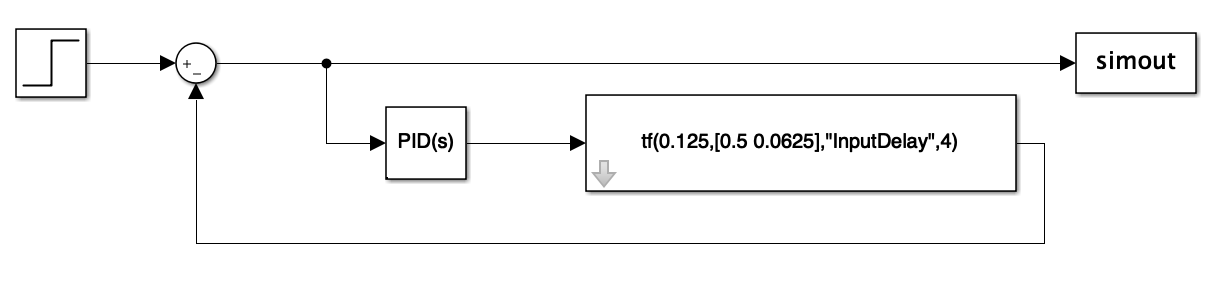
\includegraphics[width=120mm]{schemat.png}
	\caption{Schemat systemu służący do symulacji.}
    \label{fig:Rysunek}
\end{figure}

%-------------------------------------------------------------------------------------
%                                ZADANIE 2
%-------------------------------------------------------------------------------------
\subsection{Dobór optymalnego regulatora}

Przy doborze optymalnego regulatora i jego parametrów używałem poniższej funkcji napisanej w Matlabie.

%--------------
%zmieniłem trochę funkcję, żeby była czytelniejsza, z resztą i tak w większości wywoływałem ją dla 3:3,2:2, etc. ;)
%--------------
\begin{lstlisting}[caption=Funkcja testująca system.]
function testLTI(P, I, D, N, C, d)
hold on;
load_system('LTI.slx');
set_param('LTI/PID Controller1', 'P', num2str(P));   
set_param('LTI/PID Controller1', 'I', num2str(I));   
set_param('LTI/PID Controller1', 'D', num2str(D));

a=2*N/((d^2)*C);
b=1/d;
B=(C*C)/(2*N*N);

num =  B;

set_param('LTI/LTI System','SYS', ['tf(',num2str(num),',[',num2str(a+b),' ',num2str(a*b),'],"InputDelay",',num2str(d),')']);

sim('LTI.slx');
figure(1);
plot(simout.time, simout.signals.values, 'DisplayName', num2str(D));

end
\end{lstlisting}

Do testów wybrałem następujące parametry $N = 6$, $C = 3$, $d = 4$

\newpage
\subsubsection{Regulator P}

Symulując system z regulatorem P wywoływałem powyższą funkcję, podając wartość $0$ dla parametrów $I$, oraz $D$. W ten sposób uzyskałem poniższe wykresy.

\begin{figure}[!h]
    \centering
	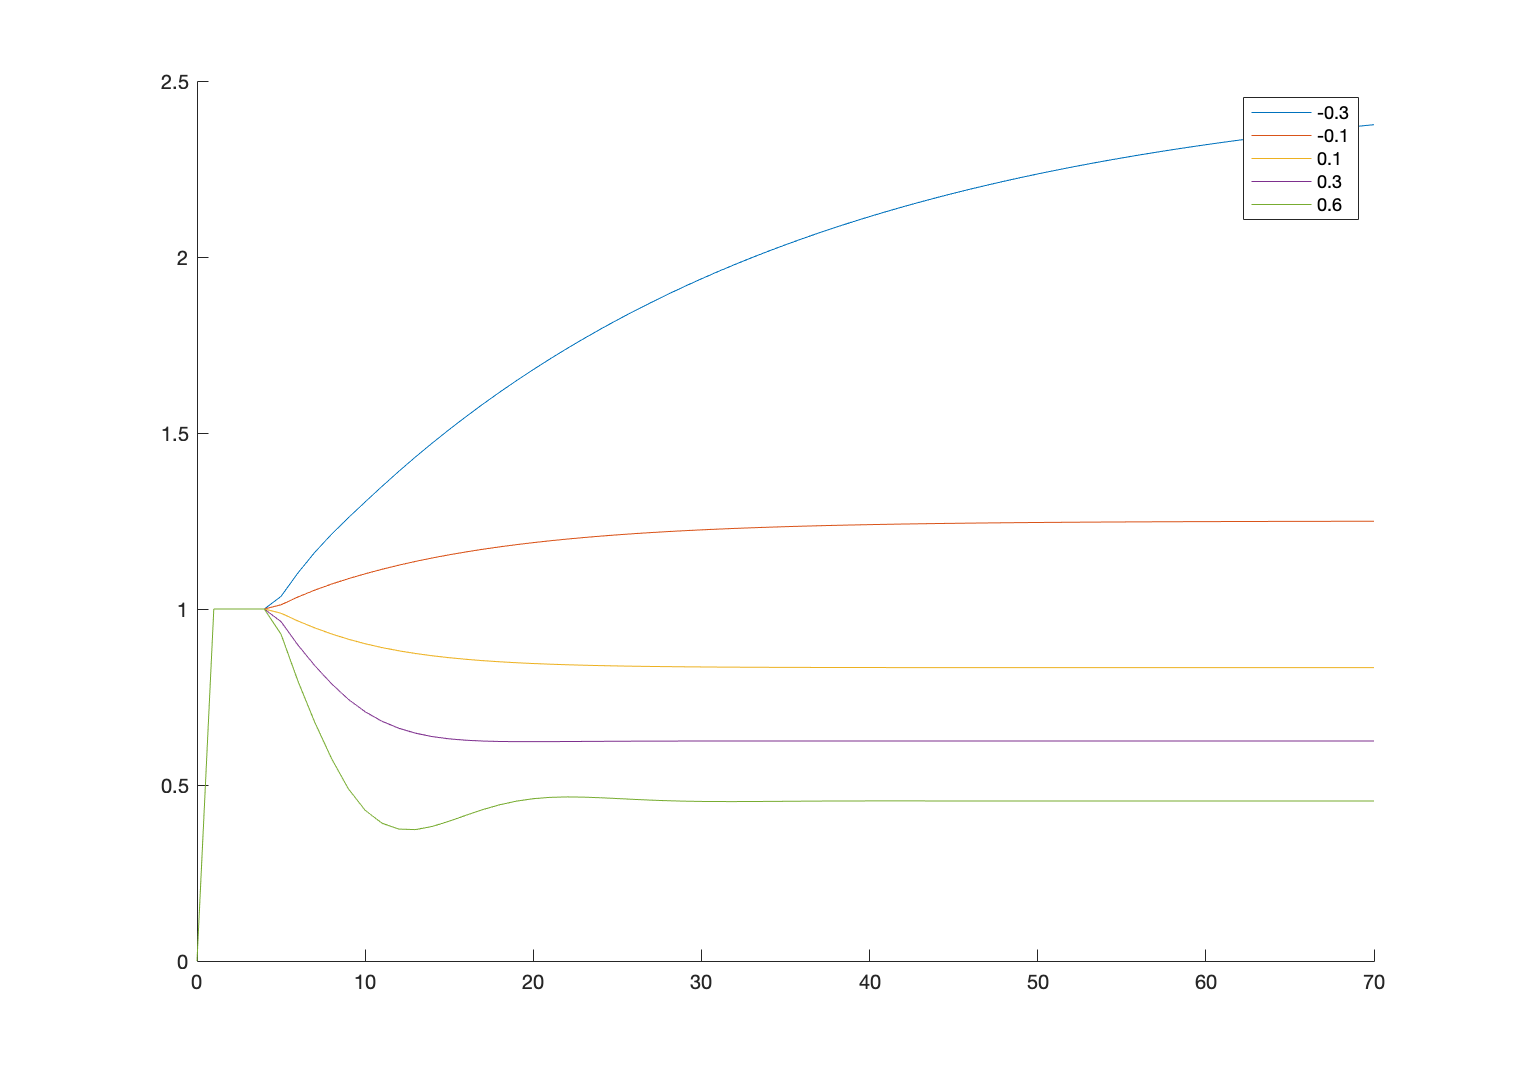
\includegraphics[width=120mm]{p_1.png}
	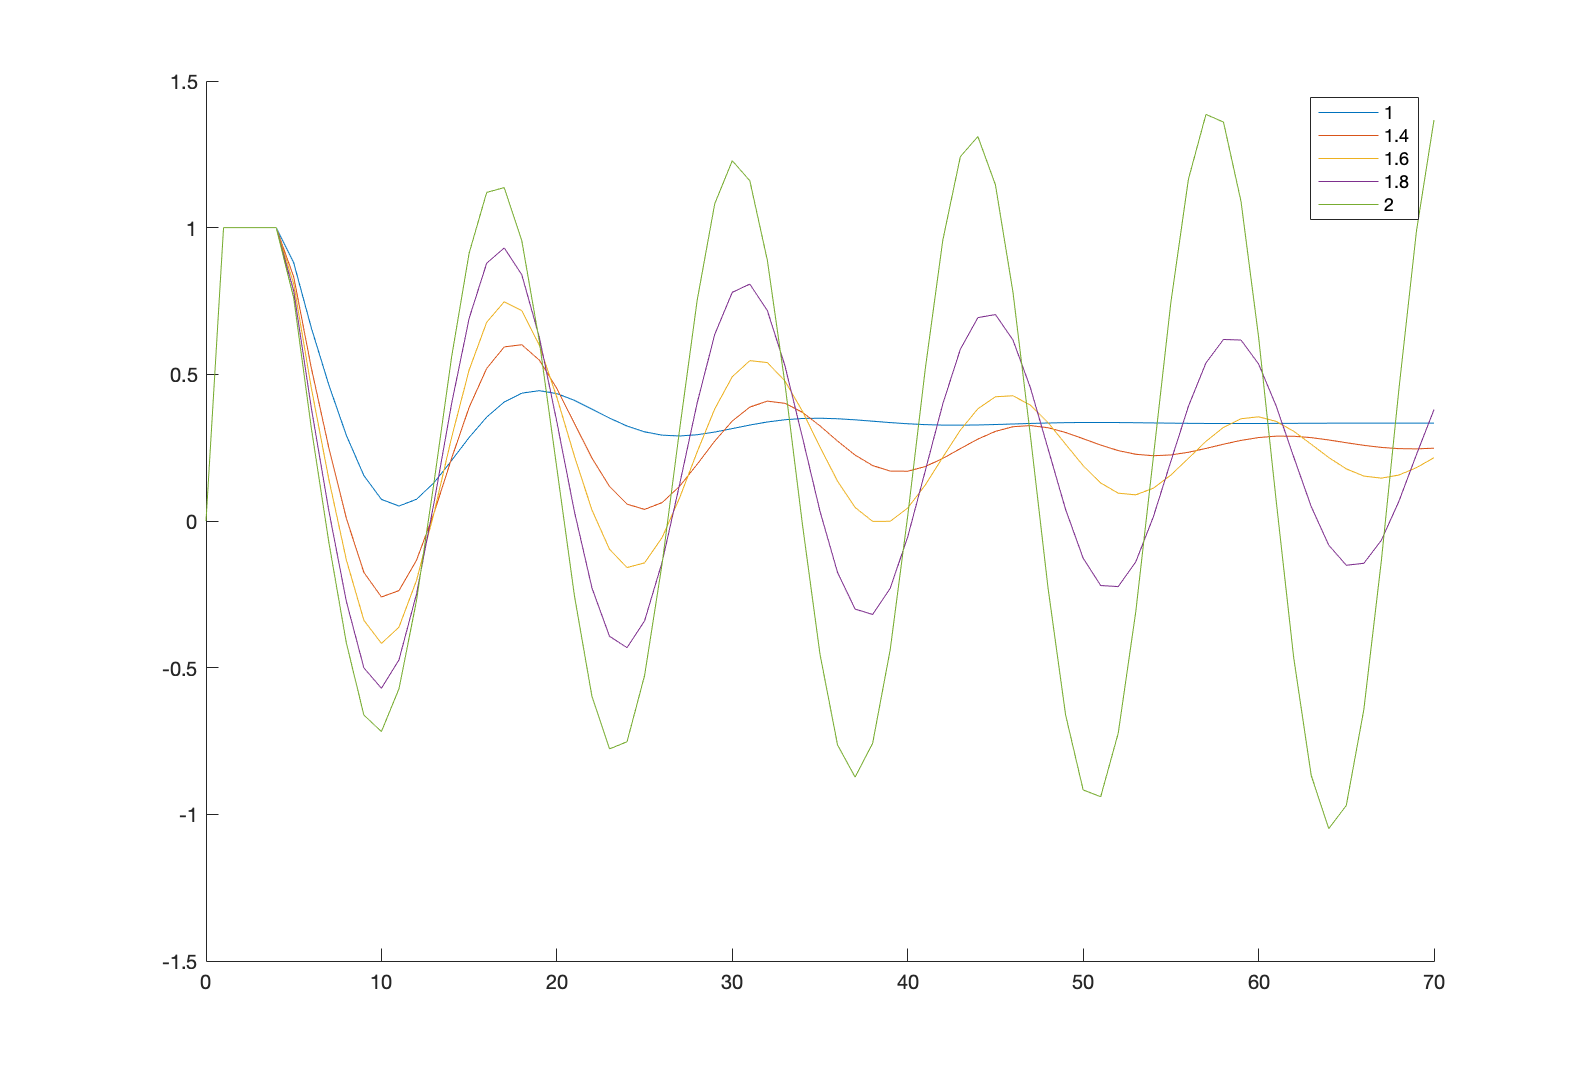
\includegraphics[width=120mm]{p_2.png}
	\caption{Wykresy przebiegu błędu regulacji przy zmianie parametru $P$}
    \label{fig:symulacjaP}
\end{figure}

\newpage

\begin{figure}[!h]
	\centering
	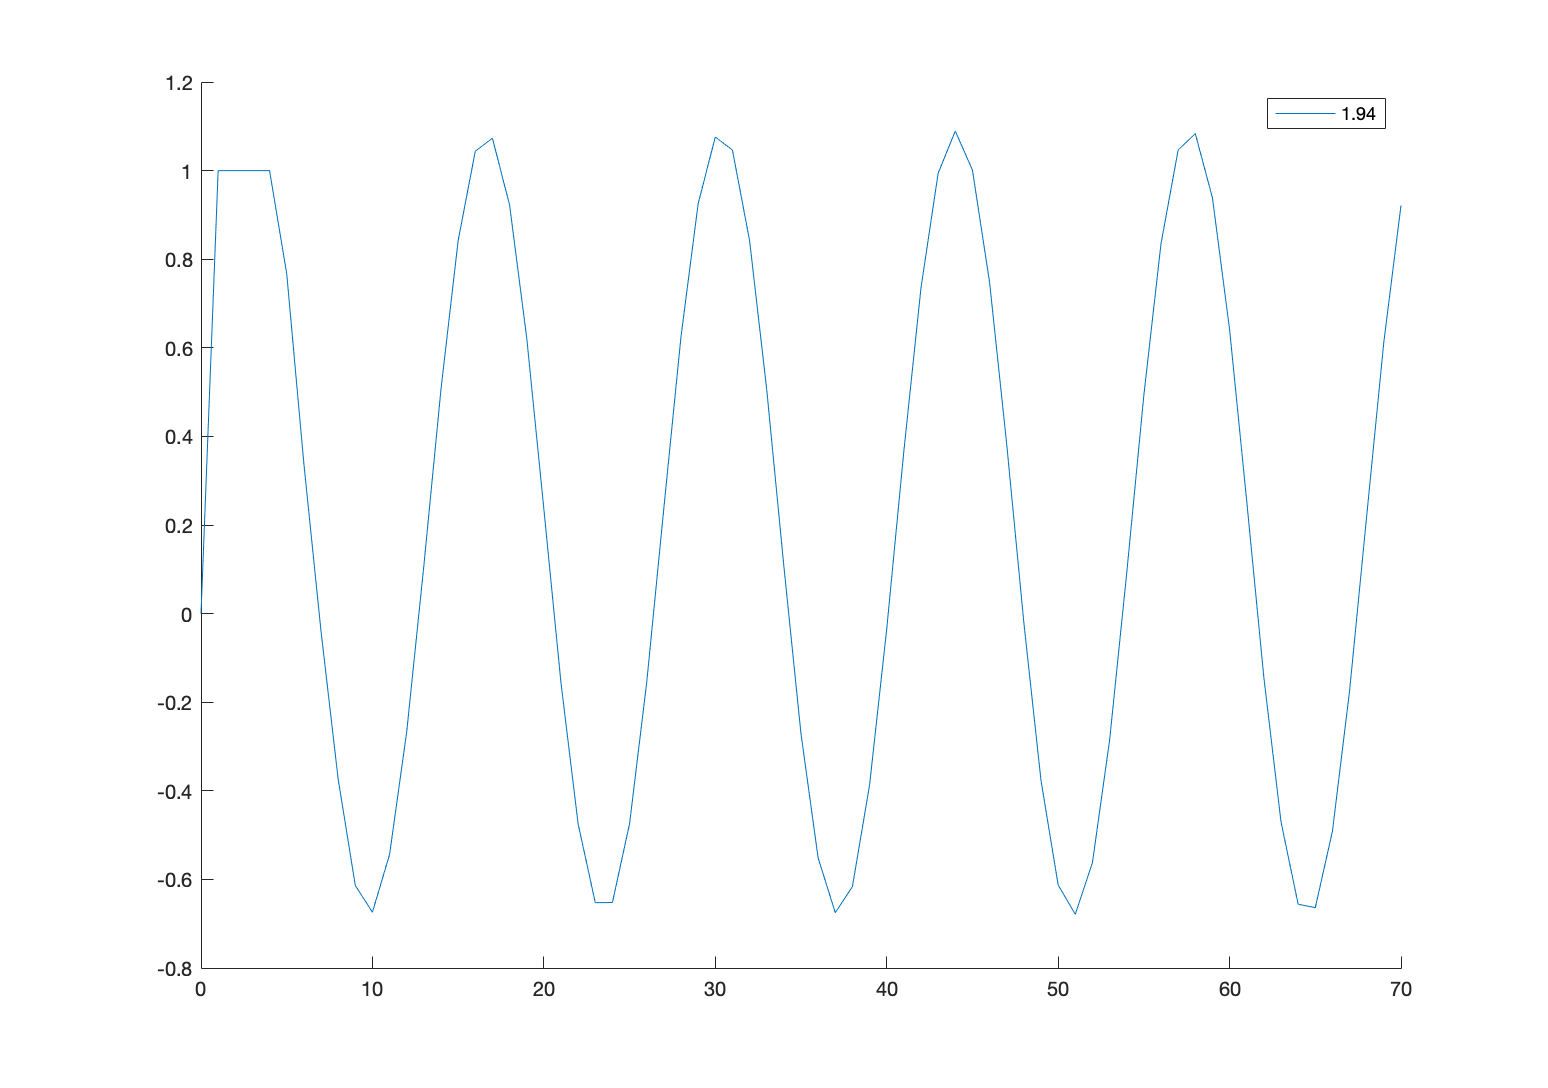
\includegraphics[width=120mm]{p_3.png}
	\caption{Wykresy przebiegu błędu regulacji dla parametru $P=1.94$}
	\label{fig:symulacjaP194}
\end{figure}

Na wykresach możemy zaobserwować, że:
\begin{itemize}
	\item Dla ujemnych wartości parametru $P$ wartość błędu szybko stabilizuje się na pewnym poziomie. Poziom ten jest tym większy, im mniejsza jest wartość parametru $P$.
	\item Dla małych ($<1.4$) dodatnich wartości parametru $P$ wartość błędu również szybko stabilizuje się na pewnym poziomie, a poziom ten jest tym mniejszy, im większa jest wartość parametru $P$.
	\item Dla większych wartości dodatnich ($>1.4$) wykres wartości błędu regulacji wolniej stabilizuje się, a dla $P \approx 1.94$ przybiera kształt drgań o stałej amplitudzie. Powyżej tej wartości amplituda drgań z czasem rośnie.
\end{itemize}
\newpage


\subsubsection{Regulator PI}
Dla regulatora PI wywołałem funkcję z parametrami $P=1.94$ oraz $D=0$.
Podobnie jak  w przypadku regulatora P, tutaj za wartość optymalną uznałęm 0.1, dla niej wykres ma prawie stałą amlitudę błędu.


\begin{figure}[!h]
	\centering
	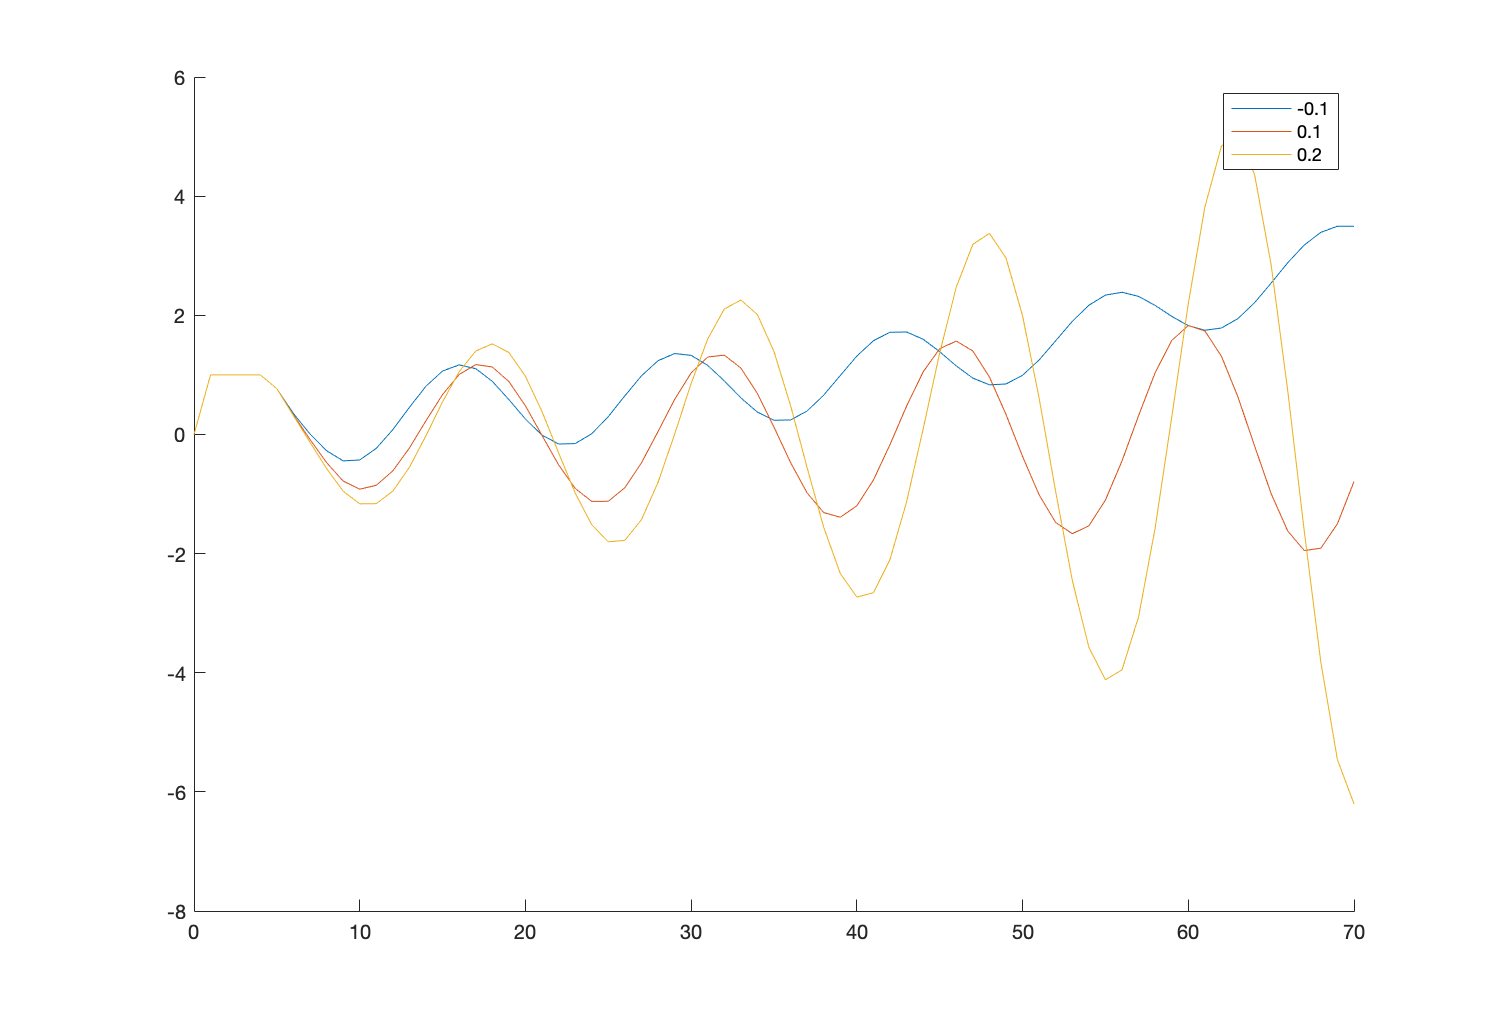
\includegraphics[width=120mm]{pi_1.png}
	\caption{Wykresy przebiegu błędu regulacji przy zmianie parametru $I$}
	\label{fig:symulacjaPI}
\end{figure}


\subsubsection{Regulator PID}
Dla regulatora PID wywołałem funkcję z parametrami $P=1.94$ oraz $I=0.1$.

\begin{figure}[!h]
    \centering
	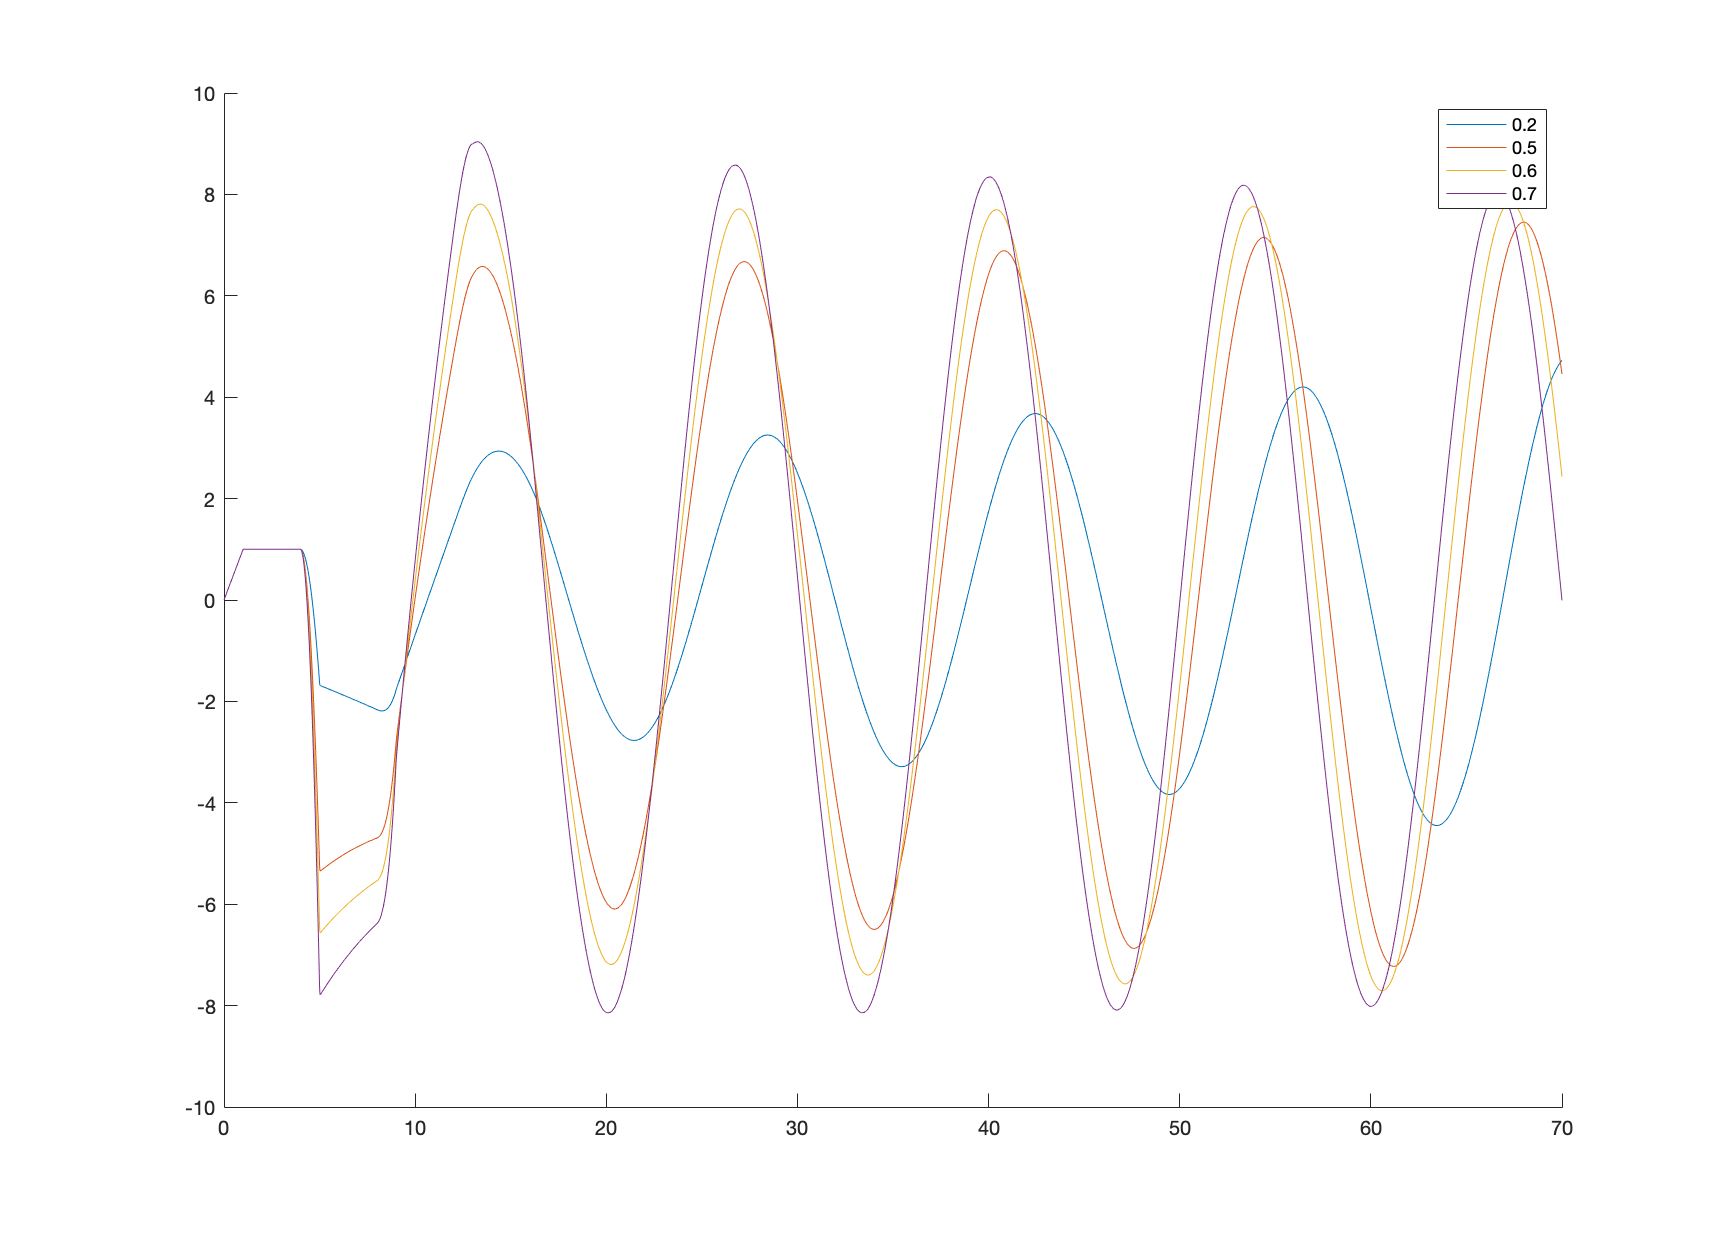
\includegraphics[width=120mm]{pid_1.png}
	\caption{Wykresy przebiegu błędu regulacji przy zmianie parametru $D$}
    \label{fig:symulacjaPID}
\end{figure}

\newpage

\begin{figure}[!h]
	\centering
	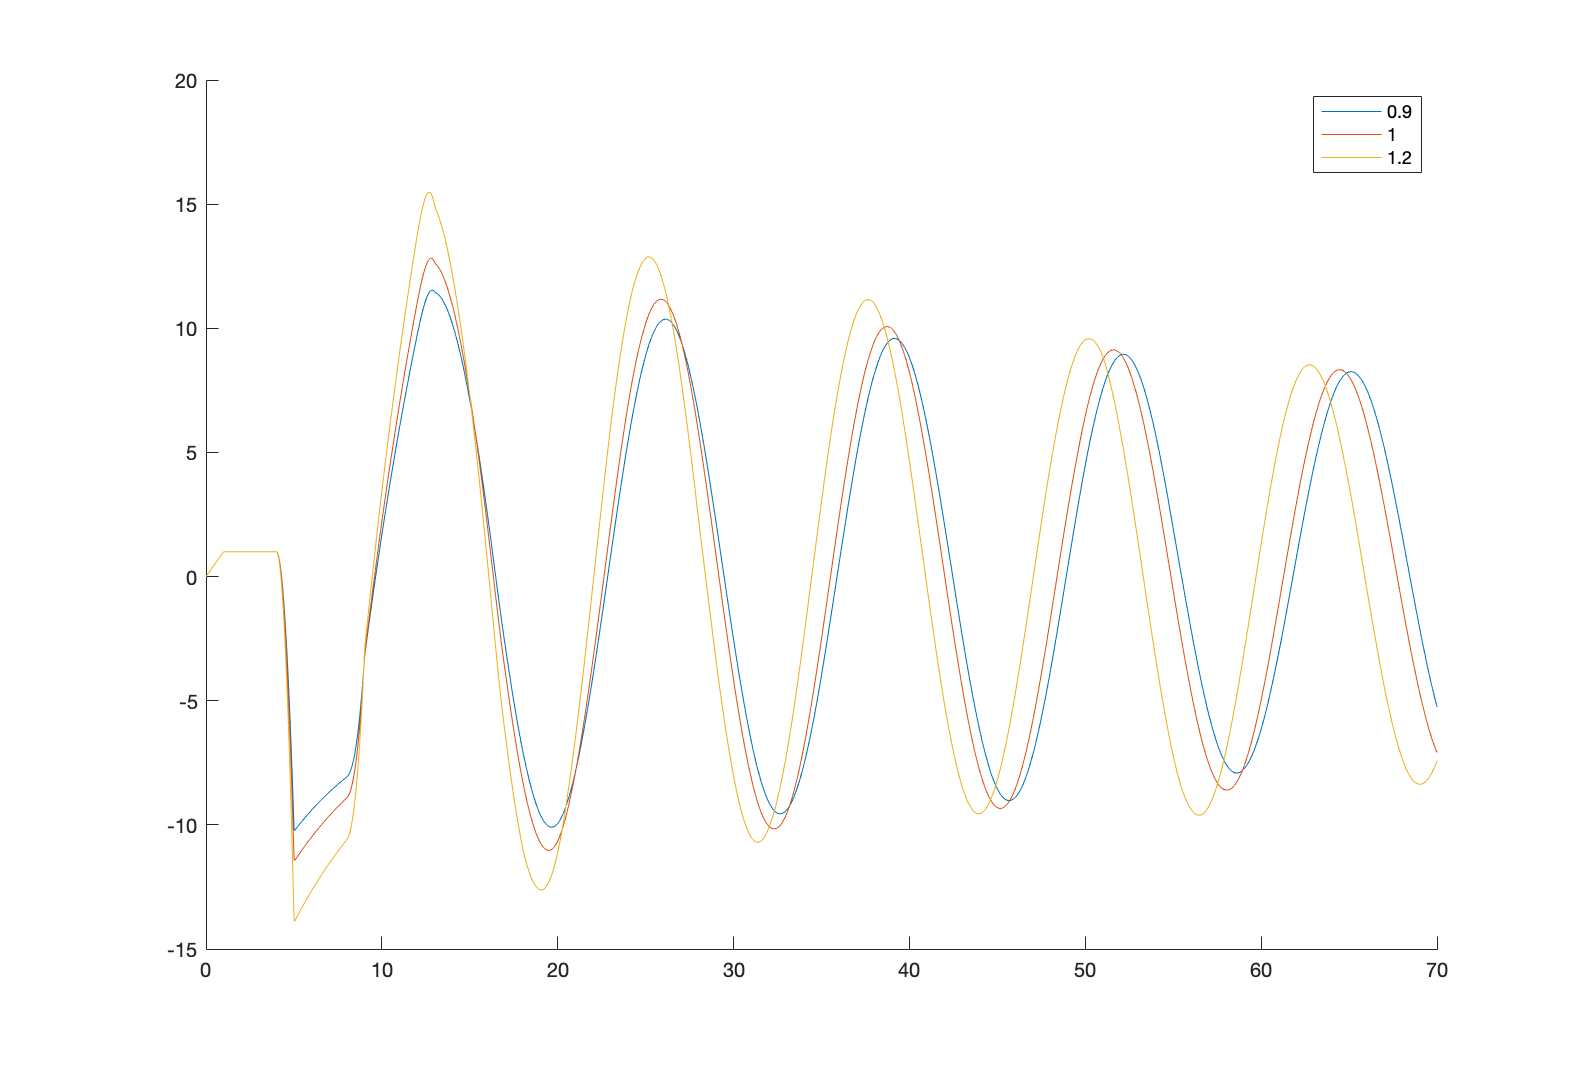
\includegraphics[width=120mm]{pid_2.png}
	\caption{Wykresy przebiegu błędu regulacji przy zmianie parametru $D$}
	\label{fig:symulacjaPID}
\end{figure}

Dla wartości poniżej 0.6 amplituda jest tym większa im mniejsza wartość, dla wartości równej 0.6 błąd ma stałą amplitudę, natomiast powyżej 0.6 amplituda maleje.


\subsubsection{Metoda Zieglera-Nicholsa}\label{sec:Mzn}
Zadanie polega na doborze parametrów regulatora PID według zasad Zieglera–
Nicholsa\\ \\
Doświadczalnie znaleźć współczynnik wzmocnienia, dla którego układ traci
stabilność. \\
$p=1.94$\\ \\
B. Ustalić okres oscylacji i wzmocnienie krytyczne.\\
$K_u=13$\\
$K_p=1.07$\\ \\
C. Według odpowiednich rekomendacji określić wartości parametrów regulatora PID. \\		
$P= K_p*0.6 = 0.642$ \\
$I= K_u*0.5 = 6.5$ \\
$D= K_u*0.125 = 1.625$ \\

\subsection{Zastosowanie członu korekcyjnego}\label{sec:zad1_P}

\subsubsection{Symulacja systemu sterowania szybkością transmisji z członem korekcyjnym}

\begin{figure}[!h]
	\centering
	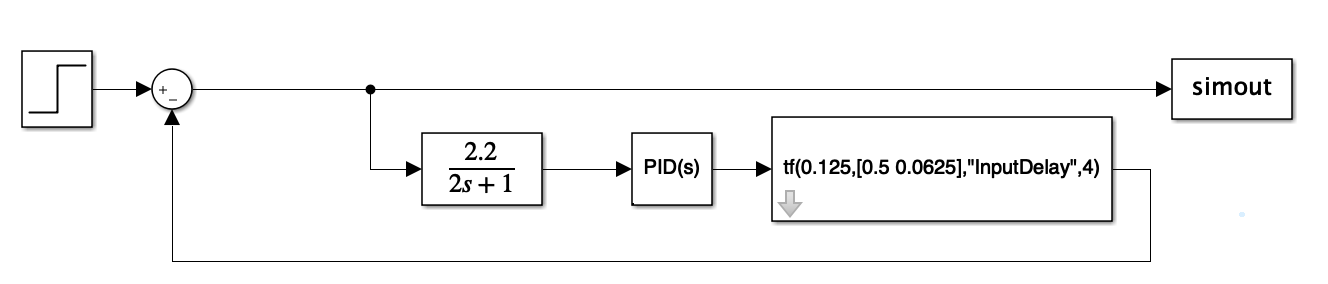
\includegraphics[width=120mm]{schemat_kor.png}
	\caption{Schemat systemu z członem korygującym}
	\label{fig:Wykres 7}
\end{figure}

\newpage
\subsubsection{Dobór optymalnych parametrów}
\begin{lstlisting}[caption=Funckja do symulacji systemu z blokiem korekcyjnym]
function testLTIKor(P, I, D, N, C, d, start, step, stop)
load_system('LTI_kor.slx');
hold on;
set_param('LTI_kor/PID Controller1', 'P', num2str(P));   
set_param('LTI_kor/PID Controller1', 'I', num2str(I));   
set_param('LTI_kor/PID Controller1', 'D', num2str(D));

a=2*N/((d^2)*C);
b=1/d;
B=(C*C)/(2*N*N); 
num =  B;
set_param('LTI_kor/LTI System','SYS', ['tf(',num2str(num),',[',num2str(a+b),' ',num2str(a*b),'],"InputDelay",',num2str(d),')']);



s=start;
while(s <= stop)
%set_param('LTI_kor/Transfer Fcn', 'Denominator', strcat('[',num2str(s), ' 1]'));
set_param('LTI_kor/Transfer Fcn', 'Denominator', strcat('[3 1]'));
set_param('LTI_kor/Transfer Fcn', 'Numerator', strcat('[',num2str(s),']'));

sim('LTI_kor.slx');
s= s+step;
figure(1);
plot(simout.time, simout.signals.values, 'DisplayName', strcat('Tk=',num2str(s)));



end
hold all;
end
\end{lstlisting}

Ustawienia parametrów: $P=1.94$, $I=0.1$, $D=0.6$, $N=6$, $C=3$, $d=4$

\begin{figure}[!h]
	\centering
	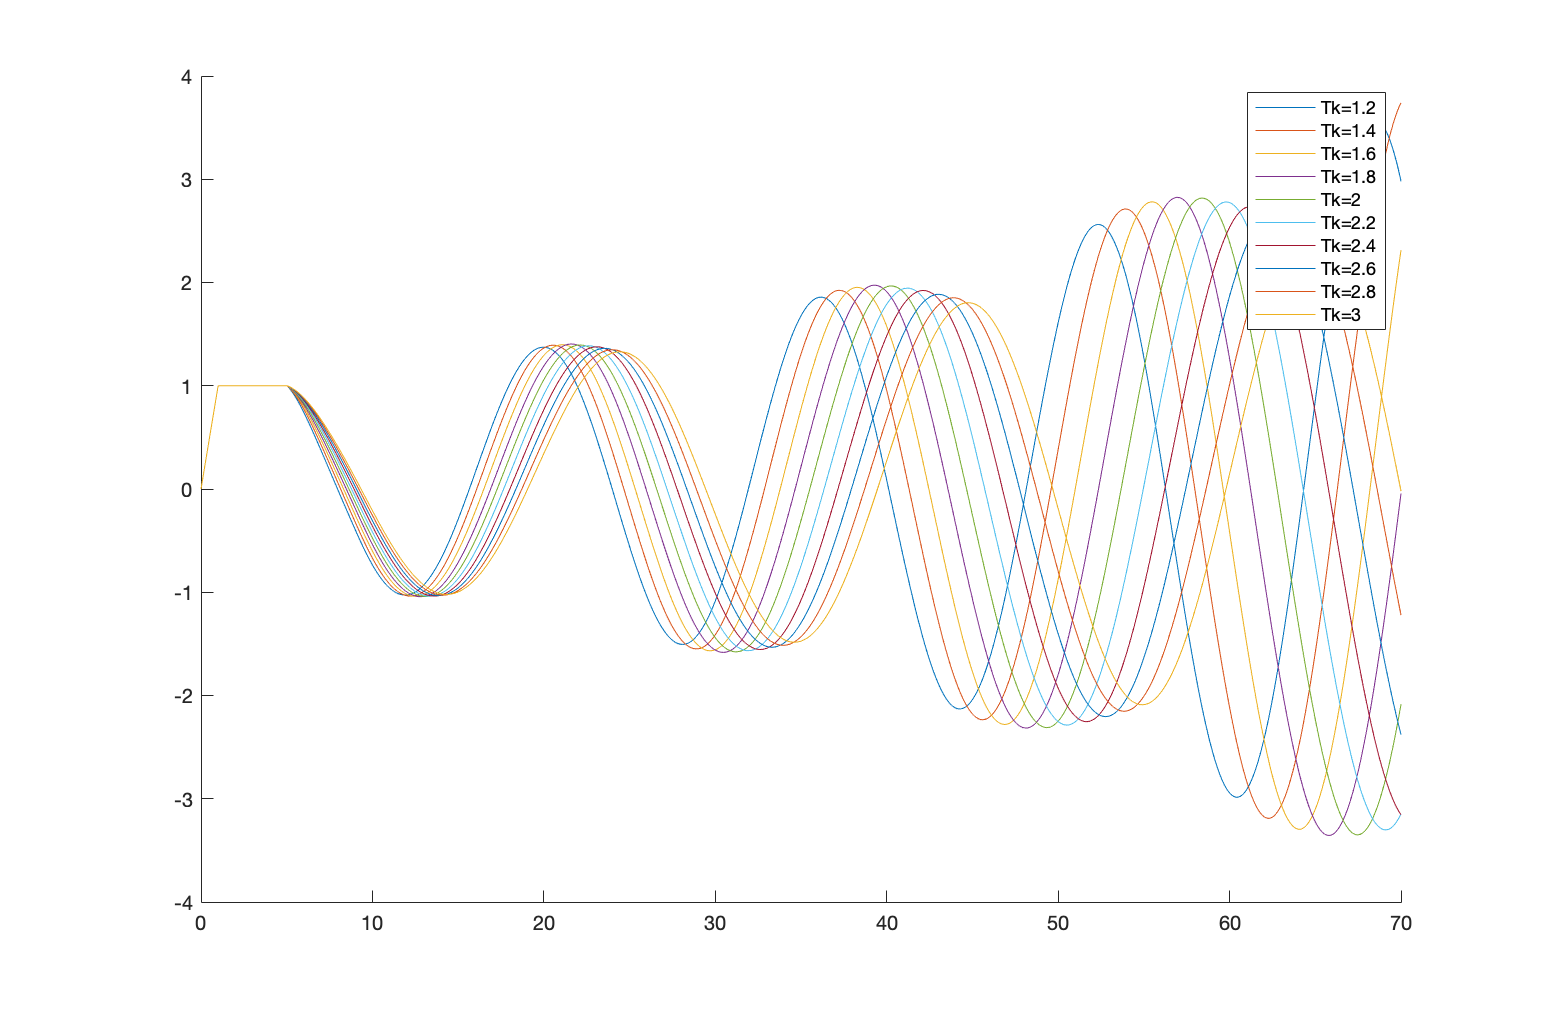
\includegraphics[width=120mm]{do_tk.png}
	\caption{Wykres błędu dla różnych wartości Tk}
	\label{fig:Wykres 8}
\end{figure}
Za optymalną wartość uznałem $Tk=3$, gdyż wtedy amplituda jest najmniejsza

\newpage

\begin{figure}[!h]
	\centering
	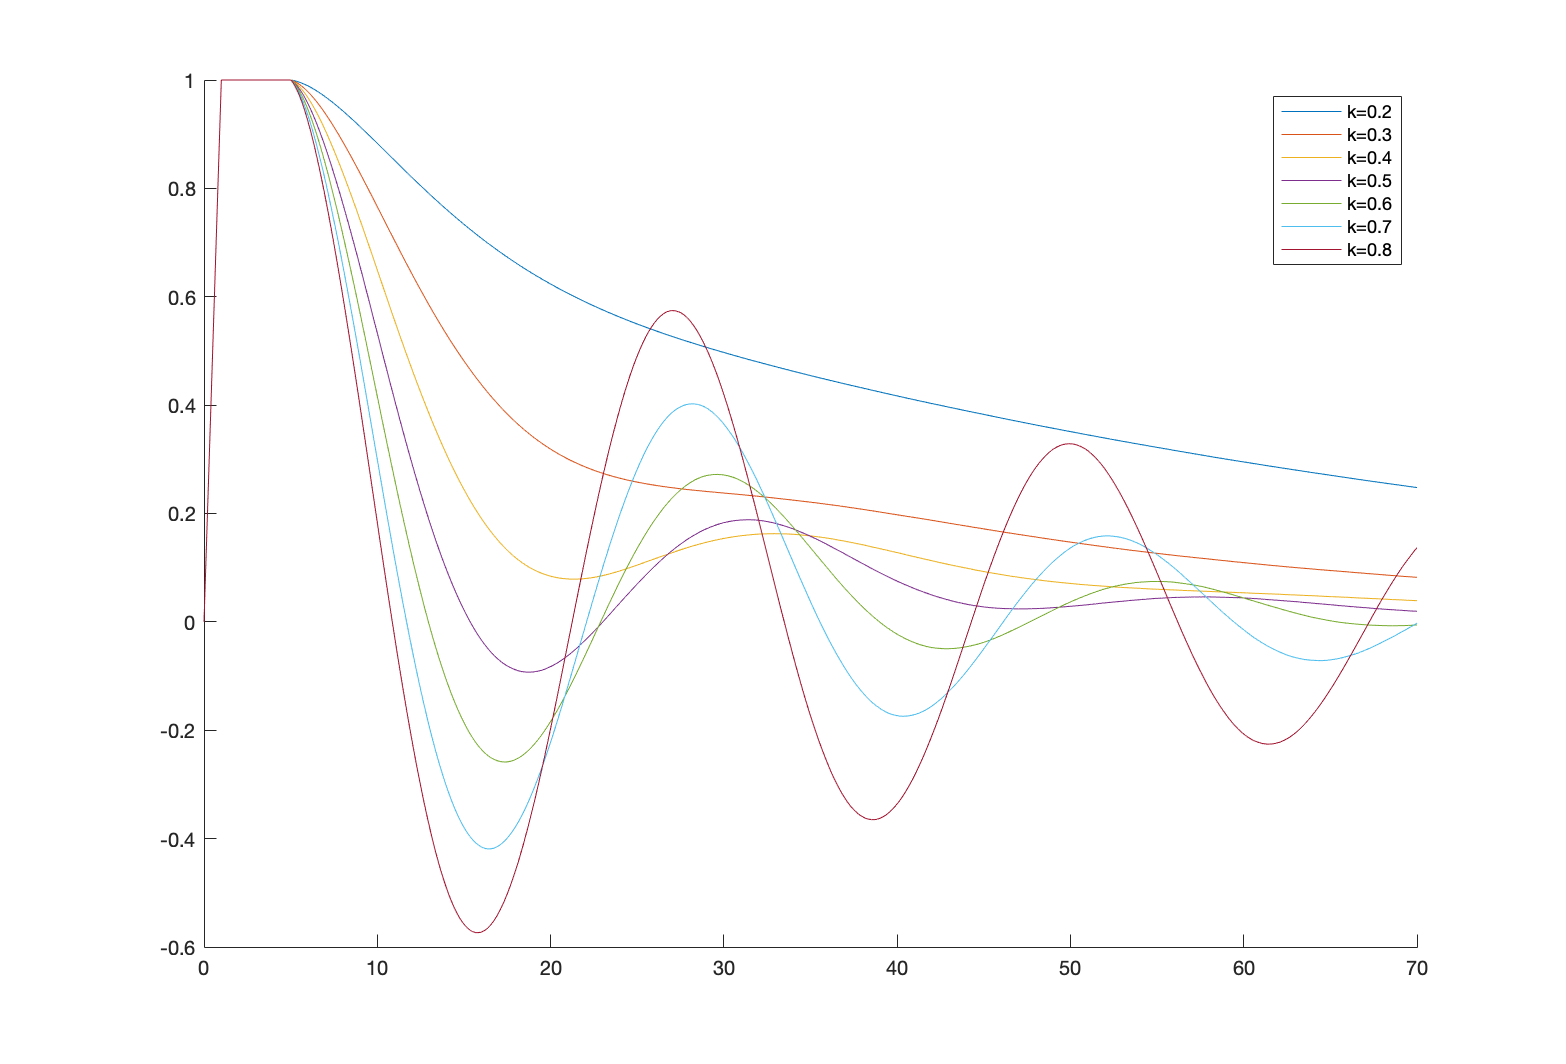
\includegraphics[width=120mm]{do_k.png}
	\caption{Wykres błędu dla różnych wartości k, przy $Tk=3$}
	\label{fig:Wykres }
\end{figure}
Za optymalną wartość uznałem  $k=0.5$, gdyż wtedy amplituda jest najmniejsza




\section{Wnioski}\label{sec:wnioski}
Z przeprowadzonego ćwiczenia wynika, że największe możliwości sterowania daje regulator PID, najbardziej można wówczas dostosować regulację do naszej funkcji. Człon korekcyjny redukuje wartość błędu. Parametry regulatora można dobrać doświaczalnie - poobnie jak w przypadku regulatorów dwu- i trójpołożeniowych.
\end{document}